\documentclass{cumcm}
\usepackage{graphicx}
\usepackage{appendix}
\numberwithin{equation}{section}
\numberwithin{equation}{subsection}
\usepackage{csvsimple}
\usepackage{listings}
\usepackage{xcolor}
%\renewcommand{\baselinestretch}{1.0}
%\newcommand{\songtiB}

% \title{text}这里是显示在第三页的文章标题
\title{\textbf{计算机系统结构实验报告\quad 实验1}\\{\Large FPGA基础实验: LED Flow Water Light}}
\author{方泓杰\ 518030910150}


\begin{document}
\maketitle

\begin{abstract}
  本实验实现了FPGA基础实验中的LED 流水灯器件。该器件在每个周期的时钟上升沿时计数器加1 ,当计数器达到最大值时,LED灯左移一位点亮;该器件还支持接收\texttt{reset}信号对LED灯进行初始化与复位。本实验通过软件仿真的形式进行实验结果的验证。
\end{abstract}

\maketitle \tableofcontents
\newpage

\section{实验目的}\label{section1}
本次实验有如下四个实验目的:
\begin{enumerate}
    \item 熟悉Xilinx逻辑设计工具Vivado的基本操作;
    \item 掌握使用VerilogHDL进行简单的逻辑设计;
    \item 理解LED流水灯的工作原理;
    \item 使用功能仿真验证功能实现的正确性。
\end{enumerate}

\section{原理分析}\label{section2}
本次实验需要实现LED流水灯这一个简单的FPGA 部件,其功能要求是每间隔一段时间点亮下一个LED灯并且熄灭当前的LED灯。我们可以利用一个计数器\texttt{cnt\_reg}实现时钟周期数目的记录,当计数器达到我们设定的最大值时,我们进行LED灯的切换,同时将计数器重置为0。由于我们使用8位LED灯,我们采取8位二进制编码\texttt{light\_reg}来表示之;第$i$位为0说明第$i$个LED灯未被点亮;第$i$位为1说明第$i$个LED灯被点亮。于是我们可以使用左移操作进行LED灯的切换;需要注意的是,如果当前点亮的是最后一个LED灯,即8位二进制编码仅最高位为1,我们需要特殊处理,将下一个状态的8位二进制编码设为仅最低一位为1,从而实现LED灯的循环点亮。此外,我们还需要设计针对\texttt{reset}信号进行重置这一特殊机制。

\section{功能实现}\label{section3}
根据第 \ref{section2} 节中所阐释的原理,我们使用计数器\texttt{cnt\_reg}实现时钟周期数目的记录,并且使用8位二进制编码\texttt{light\_reg}来表示这个8位LED灯。

我们采取如下代码实现对于计数器\texttt{cnt\_reg}的更新,并在其中加入关于重置模块的设计:当\texttt{reset}信号为1时,我们将计数器清零重置。

\begin{lstlisting}[language=verilog]
always @ (posedge clock)
    begin
        if (reset)
            cnt_reg <= 0;
        else
            cnt_reg <= cnt_reg + 1;
    end
\end{lstlisting}

我们采取如下代码实现表示LED灯的8位二进制编码\texttt{light\_reg}的更新,并在其中加入关于重置模块的设计:当\texttt{reset}信号为1时,我们将LED灯状态设为初始状态(仅点亮第一个LED灯)。

\begin{lstlisting}[language=verilog]
always @ (posedge clock)
    begin
        if (reset)
            light_reg <= 8'h01;
        else if (cnt_reg == 24'hffffff)
            begin
                if (light_reg == 8'h80)
                    light_reg <= 8'h01;
                else
                    light_reg <= light_reg << 1;
            end
    end
\end{lstlisting}

在实际的仿真验证过程中,我们发现上述设定的计数器最大值过大,使得计数器达到最大值的次数过少,LED状态改变数量过少,导致我们通过观测到LED的改变来验证程序的正确性,因此我们将计数器的最大值进行了修改,如以下代码所示。

\begin{lstlisting}[language=verilog]
always @ (posedge clock)
    begin
        if (reset)
            light_reg <= 8'h01;
        else if (cnt_reg == 2'b11)
            begin
                if (light_reg == 8'h80)
                    light_reg <= 8'h01;
                else
                    light_reg <= light_reg << 1;
            end
    end
\end{lstlisting}

完整的代码实现参见附录 \ref{appsection1}。

\section{结果验证}\label{section4}

我们使用Verilog编写激励文件,采用软件仿真的形式对于LED流水灯进行测试(代码实现参见附录 \ref{appsection2})。初始的测试结果如图 \ref{fig1} 所示(\textbf{注意:这个图对应的不是最终结果,最终结果请看下页}):

\begin{figure}[htbp]
    \centering
    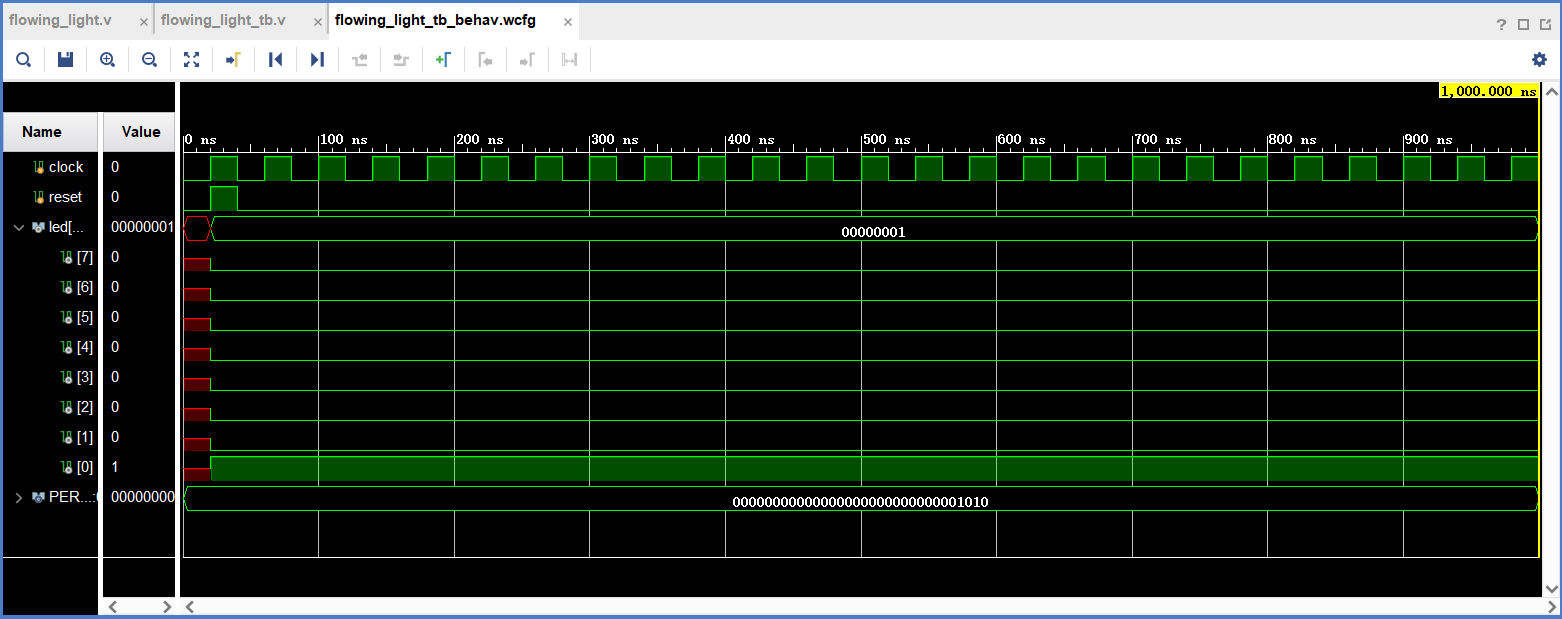
\includegraphics[width=6.3in]{1.png}
    \caption{初始测试结果}
    \label{fig1}
\end{figure}

分析该结果出现的原因,我们发现,初始设定的计数器最大值过大,使得计数器达到最大值的次数过少,LED状态改变数量过少,导致我们通过观测到LED的改变来验证程序的正确性。因此,我们对于计数器的最大值进行了一定的修改,便于我们在仿真的时候观测(这部分内容在第 \ref{section4} 节中有详细描述)。修改后的最终的测试结果如图 \ref{fig2} 所示(\textbf{注意:这个图为最终结果}):

\begin{figure}[htbp]
    \centering
    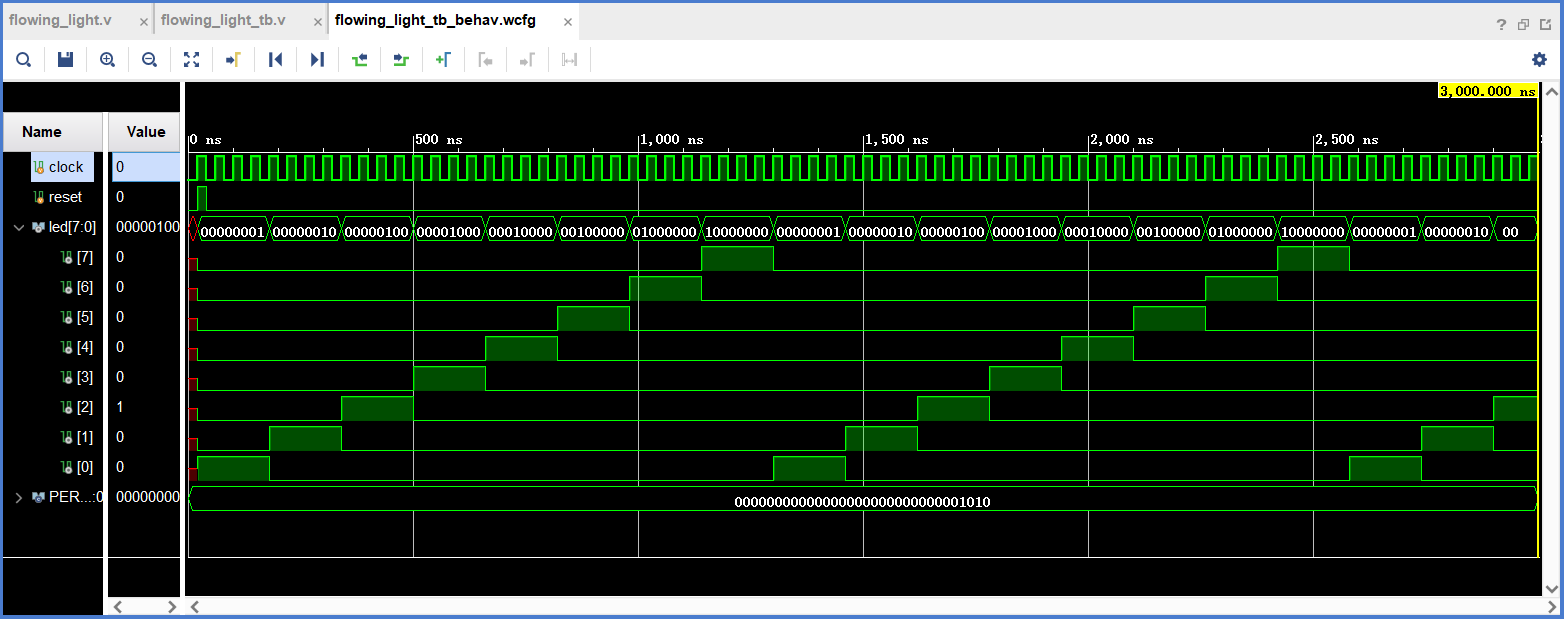
\includegraphics[width=6.3in]{2.png}
    \caption{最终测试结果}
    \label{fig2}
\end{figure}

从图 \ref{fig2} 中可以看出,我们完成了LED流水灯的功能实现,并且仿真结果正确。

\section{总结与反思}\label{section5}

本实验实现了FPGA实验中LED流水灯这一基础部件的设计与仿真。这一部件内部的逻辑较为简单,易于初学Verilog语言的编程者上手。通过这次试验,我对于Xillinx逻辑设计工具Vivado有了初步的认识,基本掌握了使用Verilog语言进行逻辑设计的方法。可以发现,Verilog语言与C语言类似,我们可以通过类比来快速掌握Verilog语言的一些基本设计方法。同时,我还学习了仿真模拟验证的具体方法。这些都为后面几次实验的复杂逻辑设计与仿真奠定了基础。观察到实验中使用了\texttt{<=}的赋值方法,我上网搜索了相关资料,发现这是时序逻辑的设计方法,而普通的赋值\texttt{=}使用的是组合逻辑的设计方法,这个认识对于后面的大型试验有着非常重要的帮助。总之,在这次实验中我收获颇丰。

\section{致谢}\label{section6}
感谢本次实验中指导老师在课程微信群里为同学们答疑解惑;

感谢上海交通大学网络信息中心提供的远程桌面资源;

感谢计算机科学与工程系相关老师对于课程指导书的编写以及对于课程的设计,让我们可以更快更好地学习相关知识,掌握相关技能;

感谢电子信息与电气工程学院提供的优秀的课程资源。
%\bibliographystyle{plain}
%\bibliography{ref}

\clearpage
\begin{appendices}
\section{设计文件完整代码实现}\label{appsection1}
参见代码文件 \texttt{flowing\_light.v}。
\section{激励文件完整代码实现}\label{appsection2}
参见代码文件 \texttt{flowing\_light\_tb.v}。
\end{appendices}

\end{document}
